En parallèle de la préemption, nous avons pu développer une gestion de la priorité. Deux possibilités s'offraient à nous : Round-robin et l'utilisation de plusieurs listes de priorités.

Round-robin consiste à voir la liste de thread $ready$ comme une liste circulaire. Tout nouveau processus est placé à la fin de la liste. Le processus courant est préempté après un temps d'exécution fonction de sa priorité, et passe la main au processus suivant.

L'autre algorithme consiste à créer une liste $ready$ pour chaque valeur de priorité. Les processus sont ajoutés à la liste correspondant à leur priorité lors de leur création. Les processus de priorités élevées sont exécutés plus souvent et plus longtemps que les autres. Pour cela, on exécute successivement un nombre défini de processus d'une liste $ready$, puis d'une autre.

\begin{figure}[!h]
\centering
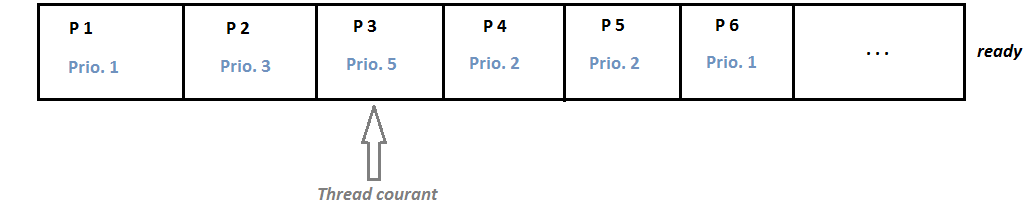
\includegraphics[width=0.9\textwidth]{round_robin.png}
\caption{Système de priorité basé sur Round-Robin}  
\label{sequence} 
\end{figure} 

\begin{figure}[!h]
\centering
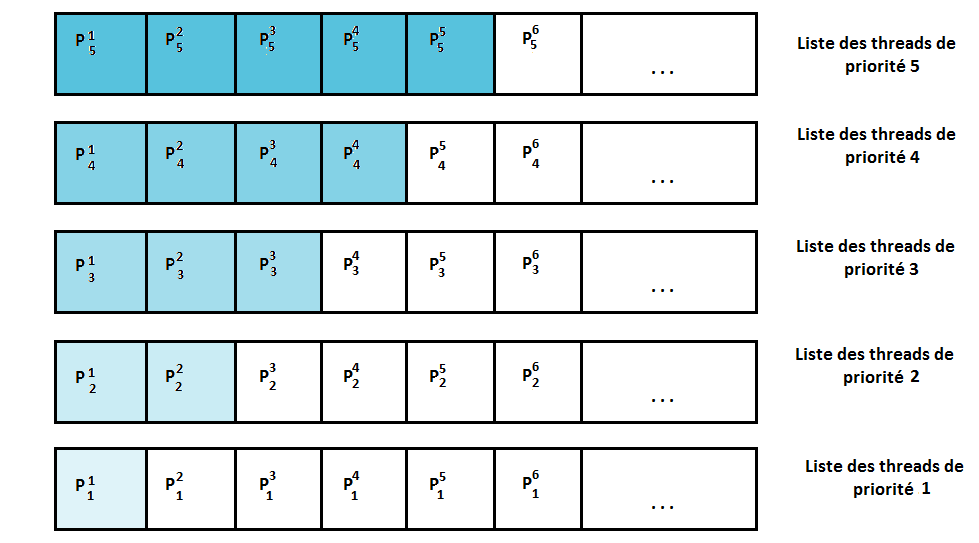
\includegraphics[width=0.9\textwidth]{queus_multi.png}
\caption{Système de priorité basé sur plusieurs listes}  
\label{sequence} 
\end{figure} 


Les deux solutions nous semblaient également efficaces (pas de famines). Nous avons cependant choisi d'implémenter Round-robin pour sa simplicité. Nous avons ajouté un champ entier $priority$ dans la structure $thread$. Plus cette priorité est élévée, plus le thread est prioritaire. Ainsi, lorsqu'un thread de $ready$ est exécuté, son temps d'exécution est proportionnel à sa priorité. Les processus de priorité s'exécutent donc plus longtemps, assurant une gestion des priorités efficace.
